\begin{figure}[htpb]
	\centering\capstart{}
	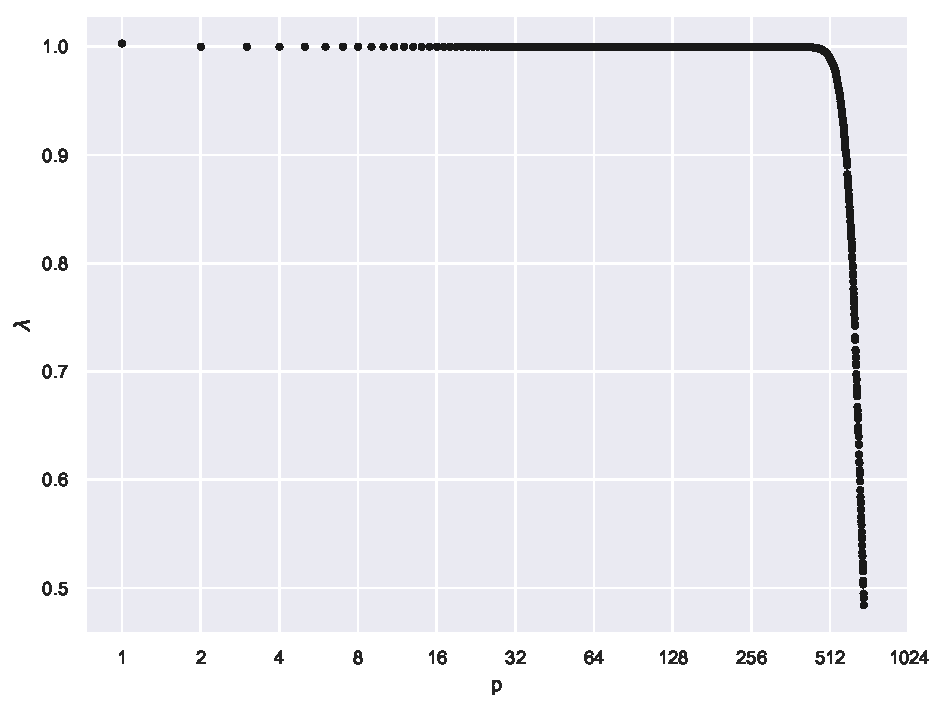
\includegraphics[width=\textwidth]{south_america_eigenvalues_L128.pdf}
	\caption[
		The Slepian eigenvalues of the South America region
	]{
		The eigenvalues of the South America region concentrated within the Shannon number \(N=690\).
		The majority of the eigenvalues are \(\almost{1}\) before decreasing rapidly towards zero around the Shannon number.
	}\label{fig:chapter3_eigenvalues}
\end{figure}
